This chapter is divided into three sections. The first section presents the results of the texture extraction for the TANDEM-X dataset and the land cover classification map obtained. The second section comprises the texture results for the SENTINEL-1 dataset and the land cover classification map. Finally, the third section presents the results of the texture extraction for the CARABAS-II dataset and the results for the proposed change detection algorithm. 

\section{Results: TANDEM-X dataset}
This section aims to assess the impact of textures in generating classification maps, i.e., whether they are useful for this purpose or not. It presents the texture results for the TANDEM-X dataset using the Sum and Difference Histogram (SADH) method, and the land cover classification map created using the texture results. Afterward, we use the texture method to improve a state-of-the-art classification map using the Rôndonia dataset acquired with the Sentinel-1 SAR system. 

\subsection{The TANDEM-X Texture Results}
It is well-known that volumetric coherence (also known as volumetric decorrelation) is the key information for creating forest maps using SAR data in the X-band \cite{Paolo,Rizzoli, Alberto}. Thus, it was chosen to extract the textural information of the volumetric coherence from the TANDEM-X dataset. An example of the volumetric coherence obtained from the TANDEM-X dataset can be seen in Figure \ref{fig:gamma_vol_tandemx}.
\begin{figure}[H]
    \centering
    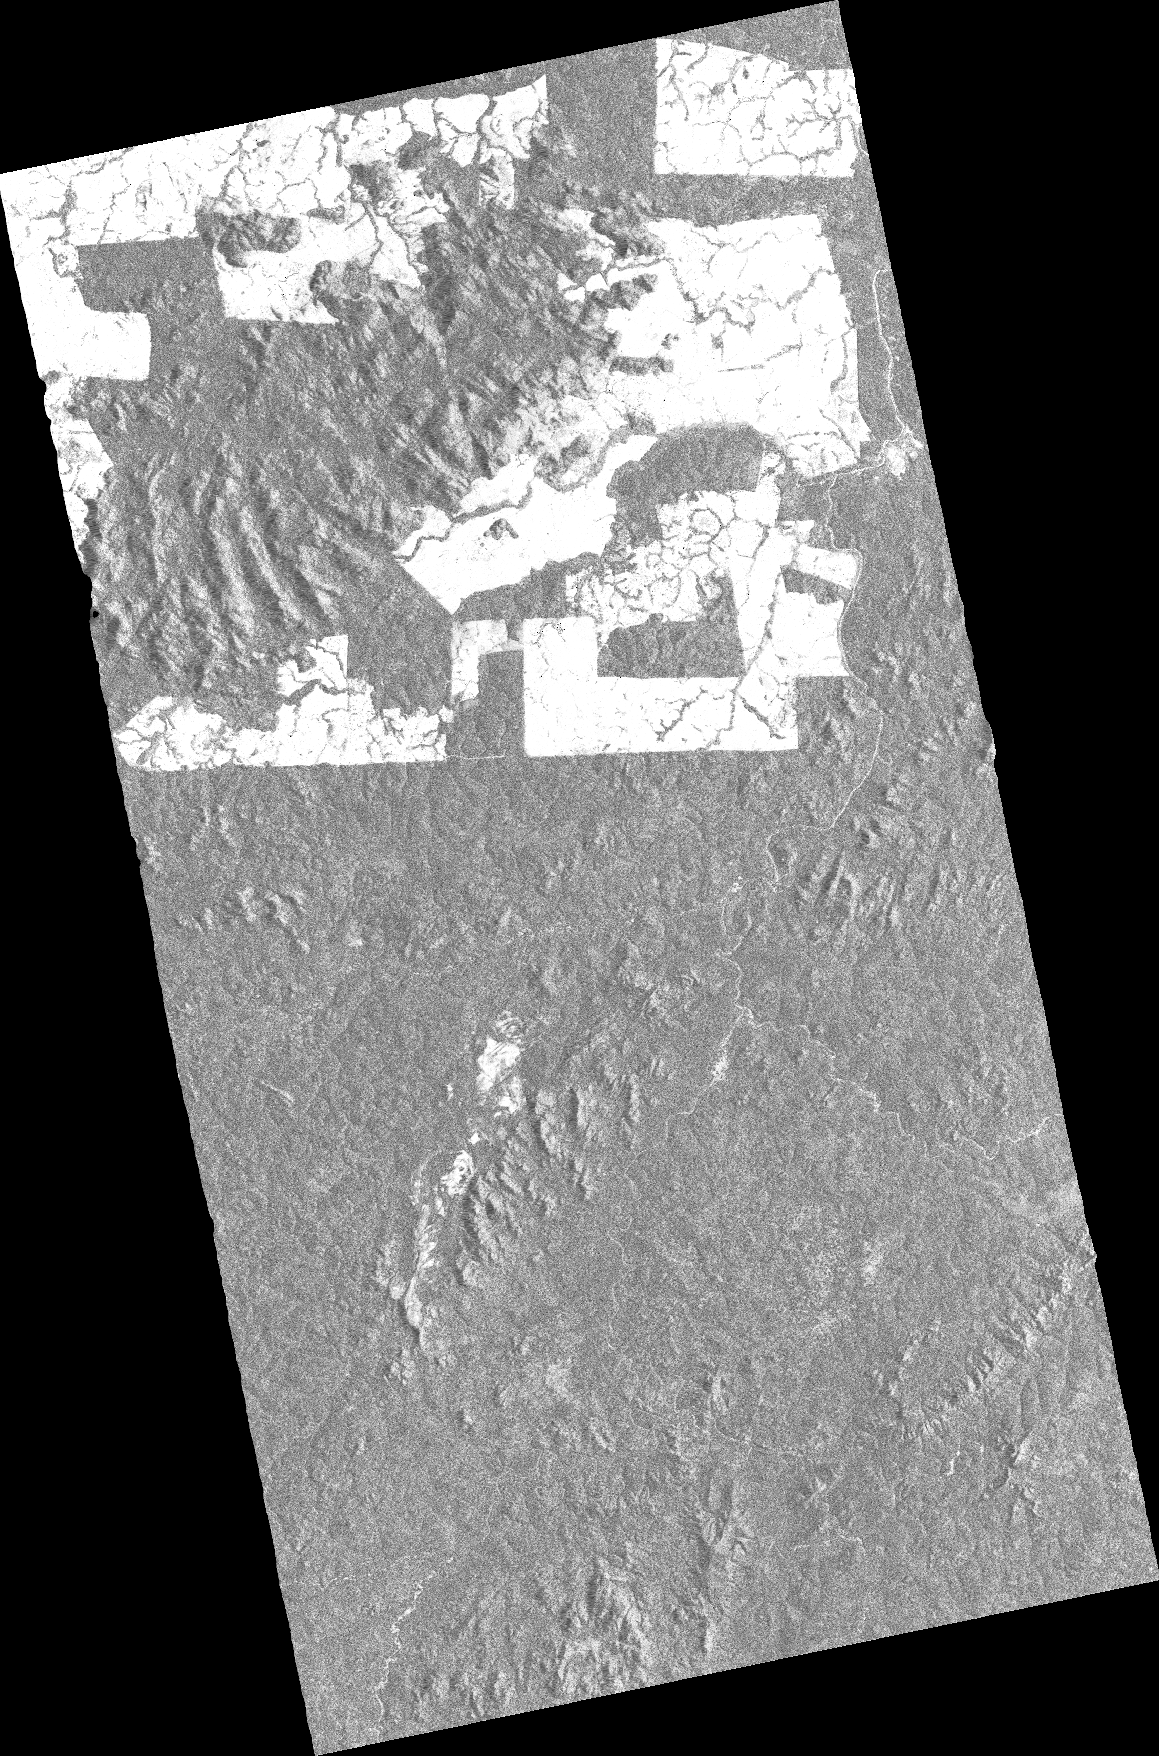
\includegraphics[width=0.7\linewidth]{Cap3-Results/coSSC_master_gamma_vol.png}
    \caption{A volumetric coherence acquisition of an area in the Amazon rainforest.}
    \label{fig:gamma_vol_tandemx}
\end{figure}

The data presented in Figure \ref{fig:gamma_vol_tandemx} is used as input for the SADH method. The obtained texture results for each image can be seen in Figure \ref{fig:tandemx_textures}. In the next section, we present the land cover classification map generated with this textural information and compare it to other available classification maps.

\begin{figure}
    \centering
    \begin{subfigure}[b]{0.4\linewidth}
      \includegraphics[width=\linewidth]{Cap3-Results/sum_and_diff_textures/cluster_prominenceimage.png}
       \caption{Cluster Prominence Texture Image}
    \end{subfigure}
    \centering
    \begin{subfigure}[b]{0.4\linewidth}
      \includegraphics[width=\linewidth]{Cap3-Results/sum_and_diff_textures/cluster_shadeimage.png}
       \caption{Cluster Shade Texture Image}
    \end{subfigure}
    \centering
    \begin{subfigure}[b]{0.4\linewidth}
      \includegraphics[width=\linewidth]{Cap3-Results/sum_and_diff_textures/contrastimage.png}
       \caption{Contrast Texture Image}
    \end{subfigure}
    \centering
    \begin{subfigure}[b]{0.4\linewidth}
      \includegraphics[width=\linewidth]{Cap3-Results/sum_and_diff_textures/correlationimage.png}
       \caption{Correlation Texture Image}
    \end{subfigure}
  \end{figure}
  \newpage
  \begin{figure}[H]\ContinuedFloat
    \centering
    \begin{subfigure}[b]{0.4\linewidth}
      \includegraphics[width=\linewidth]{Cap3-Results/sum_and_diff_textures/energyimage.png}
       \caption{Energy Texture Image}
    \end{subfigure}
    \centering
    \begin{subfigure}[b]{0.4\linewidth}
      \includegraphics[width=\linewidth]{Cap3-Results/sum_and_diff_textures/entropyimage.png}
       \caption{Entropy Texture Image}
    \end{subfigure}
    \centering
    \begin{subfigure}[b]{0.4\linewidth}
      \includegraphics[width=\linewidth]{Cap3-Results/sum_and_diff_textures/homogeneityimage.png}
       \caption{ Homogeneity Texture Image}
    \end{subfigure}
    \centering
    \begin{subfigure}[b]{0.4\linewidth}
      \includegraphics[width=\linewidth]{Cap3-Results/sum_and_diff_textures/meanimage.png}
       \caption{Mean Texture Image}
    \end{subfigure}
  \end{figure}
  \newpage
  \begin{figure}[H]\ContinuedFloat
    \centering
    \begin{subfigure}[b]{0.4\linewidth}
      \includegraphics[width=\linewidth]{Cap3-Results/sum_and_diff_textures/varianceimage.png}
       \caption{Variance Texture Image}
    \end{subfigure}
    \caption{Sum and Difference Texture Images for the TANDEM-X dataset}
    \label{fig:tandemx_textures}
  \end{figure}

\subsection{The TANDEM-X Classification Map}
We generated a classification map by combining the SADH information extracted for the TANDEM-X dataset with the original coherence image and using it as input to the Random Forest algorithm. The random forest algorithm was trained using the reference map provided by DLR. Due to computational limitations, only some textures were used: Cluster Shade, Cluster Prominence, Contrast, and Variance. Besides that, the coherence image was also given as an input to the Random Forest Algorithm. The classification results are summarized in Table \ref{tab:tandemx_results}.

\begin{table}[H]
    \centering
    \begin{tabular}{ |c |c |}
     \hline
        Textures Combination & Error Probability \\ \hline \hline
        Cluster Prominence & 3.82\% \\ \hline
        Cluster Prominence/Coherence & 3.80\% \\ \hline
        Cluster Prominence/Variance & 4.17\% \\ \hline
        Cluster Prominence/Variance/Coherence & 4.70\% \\ \hline
        Cluster Shade & 1.33\% \\ \hline
        Cluster Shade/Cluster Prominence & 1.27\% \\ \hline
        Cluster Shade/Cluster Prominence/Coherence & 1.26\% \\ \hline
        Cluster Shade/Cluster Prominence/Variance & 1.26\% \\ \hline
        Cluster Shade/Cluster Prominence/Variance/Coherence & 1.28\% \\ \hline
        Cluster Shade/Coherence & 1.30\% \\ \hline
        Cluster Shade/Variance & 1.30\% \\ \hline
        Cluster Shade/Variance/Coherence & 1.30\% \\ \hline
        Coherence & 4.70\% \\ \hline
        Contrast & 21.13\% \\ \hline
        Contrast/Cluster Prominence & 4.42\% \\ \hline
        Contrast/Cluster Prominence/Coherence & 3.47\% \\ \hline
        Contrast/Cluster Prominence/Variance & 3.81\% \\ \hline
        Contrast/Cluster Prominence/Variance/Coherence & 3.47\% \\ \hline
        Contrast/Cluster Shade & 1.30\% \\ \hline
        Contrast/Cluster Shade/Cluster Prominence & 1.15\% \\ \hline
        Contrast/Cluster Shade/Cluster Prominence/Coherence & 1.47\% \\ \hline
        Contrast/Cluster Shade/Cluster Prominence/Variance & 1.52\% \\ \hline
        Contrast/Cluster Shade/Cluster Prominence/Variance/Coherence & 1.29\% \\ 
        Contrast/Cluster Shade/Coherence & 1.30\% \\ \hline
        Contrast/Cluster Shade/Variance & 1.30\% \\ \hline
        Contrast/Cluster Shade/Variance/Coherence & 1.40\% \\ \hline
        Contrast/Coherence & 5.18\% \\ \hline
        Contrast/Variance & 21.07\% \\ \hline
        Contrast/Variance/Coherence & 4.70\% \\ \hline
        Variance/Coherence & 4.70\% \\ \hline
        Variance & 46.78\% \\ \hline
    \end{tabular}
    \caption{Probability of error of forest and deforested area classification considering different texture combinations.}
    \label{tab:tandemx_results}
\end{table}

From Table \ref{tab:tandemx_results}, it can be seen that it is possible to reduce the error probability from 4.70\% (using only the coherence image) down to 1.29\% by combining it with additional textural information such as contrast, cluster shade, cluster prominence, and variance. It is important to notice that the coherence image used is a high-quality image acquired with ideal conditions that yield a clear separation between the forest and deforested areas. However, SARs images acquired with other systems are generally not suitable for classification. The double-satellite system TANDEM-X has the advantage of not having temporal decorrelation between images since they are taken at the same time. One must also keep in mind that the frequency band of operation and image resolution are key factors for the quality of the final classification map, so one texture combination that works well in one system might not work as well as in other systems. In the next section, this method is used with images that are not suited to make a classification to assess the performance gain the textures can provide in non-ideal conditions.

\section{Results: Sentinel-1 dataset}
The Sentinel-1 dataset consists of SAR images over the Rondônia State, divided into three classes: forest, deforested, and artificial (human-made) surfaces. As mentioned in Chapter 3, the dataset consists of 12 image stacks, 8 used for Random Forest training (which used PRODES classification reference map \cite{prodes}), and four for validation purposes. The Sentinel-1 dataset is not as well suited for making forest classification maps as the TANDEM-X dataset. Thus, we use texture methods to improve the classification performance. The results are assessed in terms of overall accuracy, i.e., the number of pixels that were correctly classified divided by the number of pixels in the dataset. For explanations about different accuracy measures, such as average accuracy, precision, recall, and F-score, the reader is referred to \cite{Book_ML}.

To generate a classification map, the state-of-the-art method is used to create forest maps using Sentinel-1 data as described in \cite{Paolo}. The state-of-the-art method uses a combination of radar brightness in the plane perpendicular to the line of sight ($\gamma^0$ coefficient), incidence angle ($\theta_{inc}$), long-term coherence term ($\rho_{LT}$), and temporal decorrelation constant ($\tau$). This method is run for the Sentinel-1 dataset without the textural information and with the additional textural information. The overall accuracy results are compared to assess the impact that the texture information can make in creating classification maps.

It was obtained 18 texture results organized in two groups with nine results. The texture information was generated by the SADH method using the displacement vector equal to 1 unit in the horizontal (9 textures results) and vertical (9 textures results) directions. As a reminder, the texture information that SADH methods can create are average, cluster shade, cluster, prominence, contrast, correlation, energy, entropy, homogeneity, and variance.

The classification results for the 4 validation stacks (defined in Table \ref{tab:sentinelStackTable}) of the Sentinel-1 dataset can be seen in Figure \ref{img:sentinel_results}.

\begin{figure}
    \centering
    \includegraphics[width=0.9\linewidth]{Cap3-Results/sentinel1-classificationresults.jpg}
    \caption{Comparison between the PRODES reference map (left) and the final results of the Random Forest algorithm using SADH textures (right). The white square identifies a region of interest in which the maps are clearly different.
    Such an area corresponds to the Pacaás Novos National Park.}
    \label{img:sentinel_results}
\end{figure}

The overall accuracy (OA) for each image stack can be seen in Table \ref{tab:sentinel_table_results}.

\begin{table}[H]
    \centering
    \begin{tabular}{ |c |c | c|}
     \hline
        Image Stack & Original OA & SADH OA\\ \hline \hline
        Stack 6 & 88.48 \% & 91.90 \% \\ \hline
        Stack 7 & 82.50 \% & 84.26 \% \\ \hline
        Stack 8 & 85.03 \% & 86.49 \% \\ \hline
        Stack 9 & 84.84 \% & 87.66 \% \\  \hline
    \end{tabular}
    \caption{Overall accuracy for the four image stacks presented in Figure \ref{img:sentinel_results}.}
    \label{tab:sentinel_table_results}
\end{table}

From Table \ref{tab:sentinel_table_results}, we can see an improvement in the overall accuracy of the land cover classification map, even if the gain is not as significant as the improvement for the TANDEM-X dataset. Still, the gain is not negligible. Considering that additional texture information can be easily added to any machine learning algorithm, these results demonstrate that using textures might improve the performance of every algorithm that tries to create more accurate land cover classification maps.

\section{Results: CARABAS-II dataset}

The CARABAS-II dataset consists of 24 images of forests in northern Sweden with 25 vehicles hidden under the foliage. The objective is to detect the position of the vehicles. The dataset was organized for the change detection approach. The objective is to maximize the detection of target positions considering the changes between acquisitions and minimize the false alarm rate of such a method.
The proposed CDA algorithm is based on a 3-dimensional image tensor, one of which is the original acquisition; the other two are textures extracted using the SADH method -- the textures chosen were the entropy and the variance. The proposed CDA is based on the UNET convolutional neural network, which used 12 out of the 24 images for training purposes. One example of a CARABAS-II SAR image and two textures obtained from that image can be seen in Figures \ref{fig:carabas_example}, \ref{fig:entropy_example}, \ref{fig:variance_example}.

\begin{figure}[H]
  \centering
  \includegraphics[width=0.8\linewidth]{Cap3-Results/exemplo_carabas.jpg}
  \caption{Example of a SAR image acquired by the CARABAS-II system.
  The red circle shows the position of the cars hidden under the canopy of trees.}
  \label{fig:carabas_example}
\end{figure}

\begin{figure}[H]
  \centering
  \includegraphics[width=0.8\linewidth]{Cap3-Results/entropy_example.png}
  \caption{Entropy texture image of Figure \ref{fig:carabas_example}.
  The red circle shows the position of the cars hidden under the canopy of trees.}
  \label{fig:entropy_example}
\end{figure}

\begin{figure}[H]
  \centering
  \includegraphics[width=0.8\linewidth]{Cap3-Results/variance_exemplo.png}
  \caption{Variance texture image of Figure \ref{fig:carabas_example}.
  The red circle shows the position of the cars hidden under the canopy of trees.}
  \label{fig:variance_example}
\end{figure}

After running the CDA algorithm proposed in Section 3, we selected 24 pairs of images to assess the quality of the change detection algorithm -- the 24 pairs selected followed the standard selection used for CDA testing and validation of the CARABAS-II dataset as done in \cite{Carabas, Ricardo, LucasRamos}. One output of the proposed CDA can be seen in Figure \ref{fig:carabas_results}.

\begin{figure}[H]
  \centering
  \includegraphics[width=0.8\linewidth]{Cap3-Results/results_carabas.png}
  \caption{Results for proposed CDA. The black pixels represent non-changes, and the white pixels represent detected changes (the vehicles whose positions have been changed). All 25 vehicles were detected.}
  \label{fig:carabas_results}
\end{figure}

\begin{table}[h]
  \centering
  \begin{tabular}{|c|c||c|c|c|c|}
       \hline
       \vtop{\hbox{\strut Monitored}\hbox{\strut Image}} &
       \vtop{\hbox{\strut Reference}\hbox{\strut Image}}
       &\vtop{\hbox{\strut \vtop{\hbox{\strut Detected}\hbox{\strut Targets}}}\hbox{\strut \vtop{\hbox{\strut (with}\hbox{\strut texture)}}}}
       &\vtop{\hbox{\strut \vtop{\hbox{\strut False}\hbox{\strut Alarms}}}\hbox{\strut \vtop{\hbox{\strut (with}\hbox{\strut texture)}}}}
       &\vtop{\hbox{\strut \vtop{\hbox{\strut Detected}\hbox{\strut Targets}}}\hbox{\strut \vtop{\hbox{\strut (without}\hbox{\strut texture)}}}}
       &\vtop{\hbox{\strut \vtop{\hbox{\strut False}\hbox{\strut Alarms}}}\hbox{\strut \vtop{\hbox{\strut (without}\hbox{\strut texture)}}}}
       \\
       \hline \hline
       2\_1&3\_1&25&0&25&0\\
       3\_1&4\_1&23&1&21&1\\
       4\_1&5\_1&25&0&25&0\\
       5\_1&2\_1&25&0&25&0\\
       \hline
       2\_2&4\_2&25&0&25&0\\
       3\_2&5\_2&25&0&23&1\\
       4\_2&2\_2&23&0&25&0\\
       5\_2&3\_2&22&0&24&0\\
       \hline
       2\_3&5\_3&25&0&25&0\\
       3\_3&2\_3&22&1&21&1\\
       4\_3&3\_3&25&1&25&1\\
       5\_3&4\_3&25&0&25&0\\
       \hline
       2\_4&3\_4&25&0&25&0\\
       3\_4&4\_4&24&0&23&1\\
       4\_4&5\_4&25&0&25&0\\
       5\_4&2\_4&24&0&25&0\\
       \hline
       2\_5&4\_5&25&0&25&0\\
       3\_5&5\_5&24&0&21&2\\
       4\_5&2\_5&25&0&25&0\\
       5\_5&3\_5&23&0&24&0\\
       \hline
       2\_6&5\_6&25&0&25&0\\
       3\_6&2\_6&23&1&25&0\\
       4\_6&3\_6&24&0&25&0\\
       5\_6&4\_6&25&1&25&0\\
       \hline
  \end{tabular}
  \caption{
    Results of CDA in terms of detected targets and false alarm rate for the same image pairs considered in ((LUNDBERG et al., 2006b)). It also presents the results when textural information is either used or not used as input of the proposed algorithm.}
\end{table}